\section{Interfaccia utente}
\label{sec:userInterface}
L'interfaccia utente è il luogo d'incontro tra il sistema distribuito e l'utilizzatore finale. In questo elaborato di tesi, come detto in precedenza, l'utente che vuole utilizzare e controllare i risultati del sistema distribuito deve utilizzare un qualsiasi browser e digitare l'indirizzo web del server di Blockchain explorer. L'utente dunque da qualsiasi tipo di dispositivo può accedere alla home page del portale ed iniziare ad utilizzare il sistema.
\\L'immagine \ref{fig:homePage} mostra la prima schermata che l'utente visualizza quando accede al portale.
\begin{figure}[H]
	\centering
	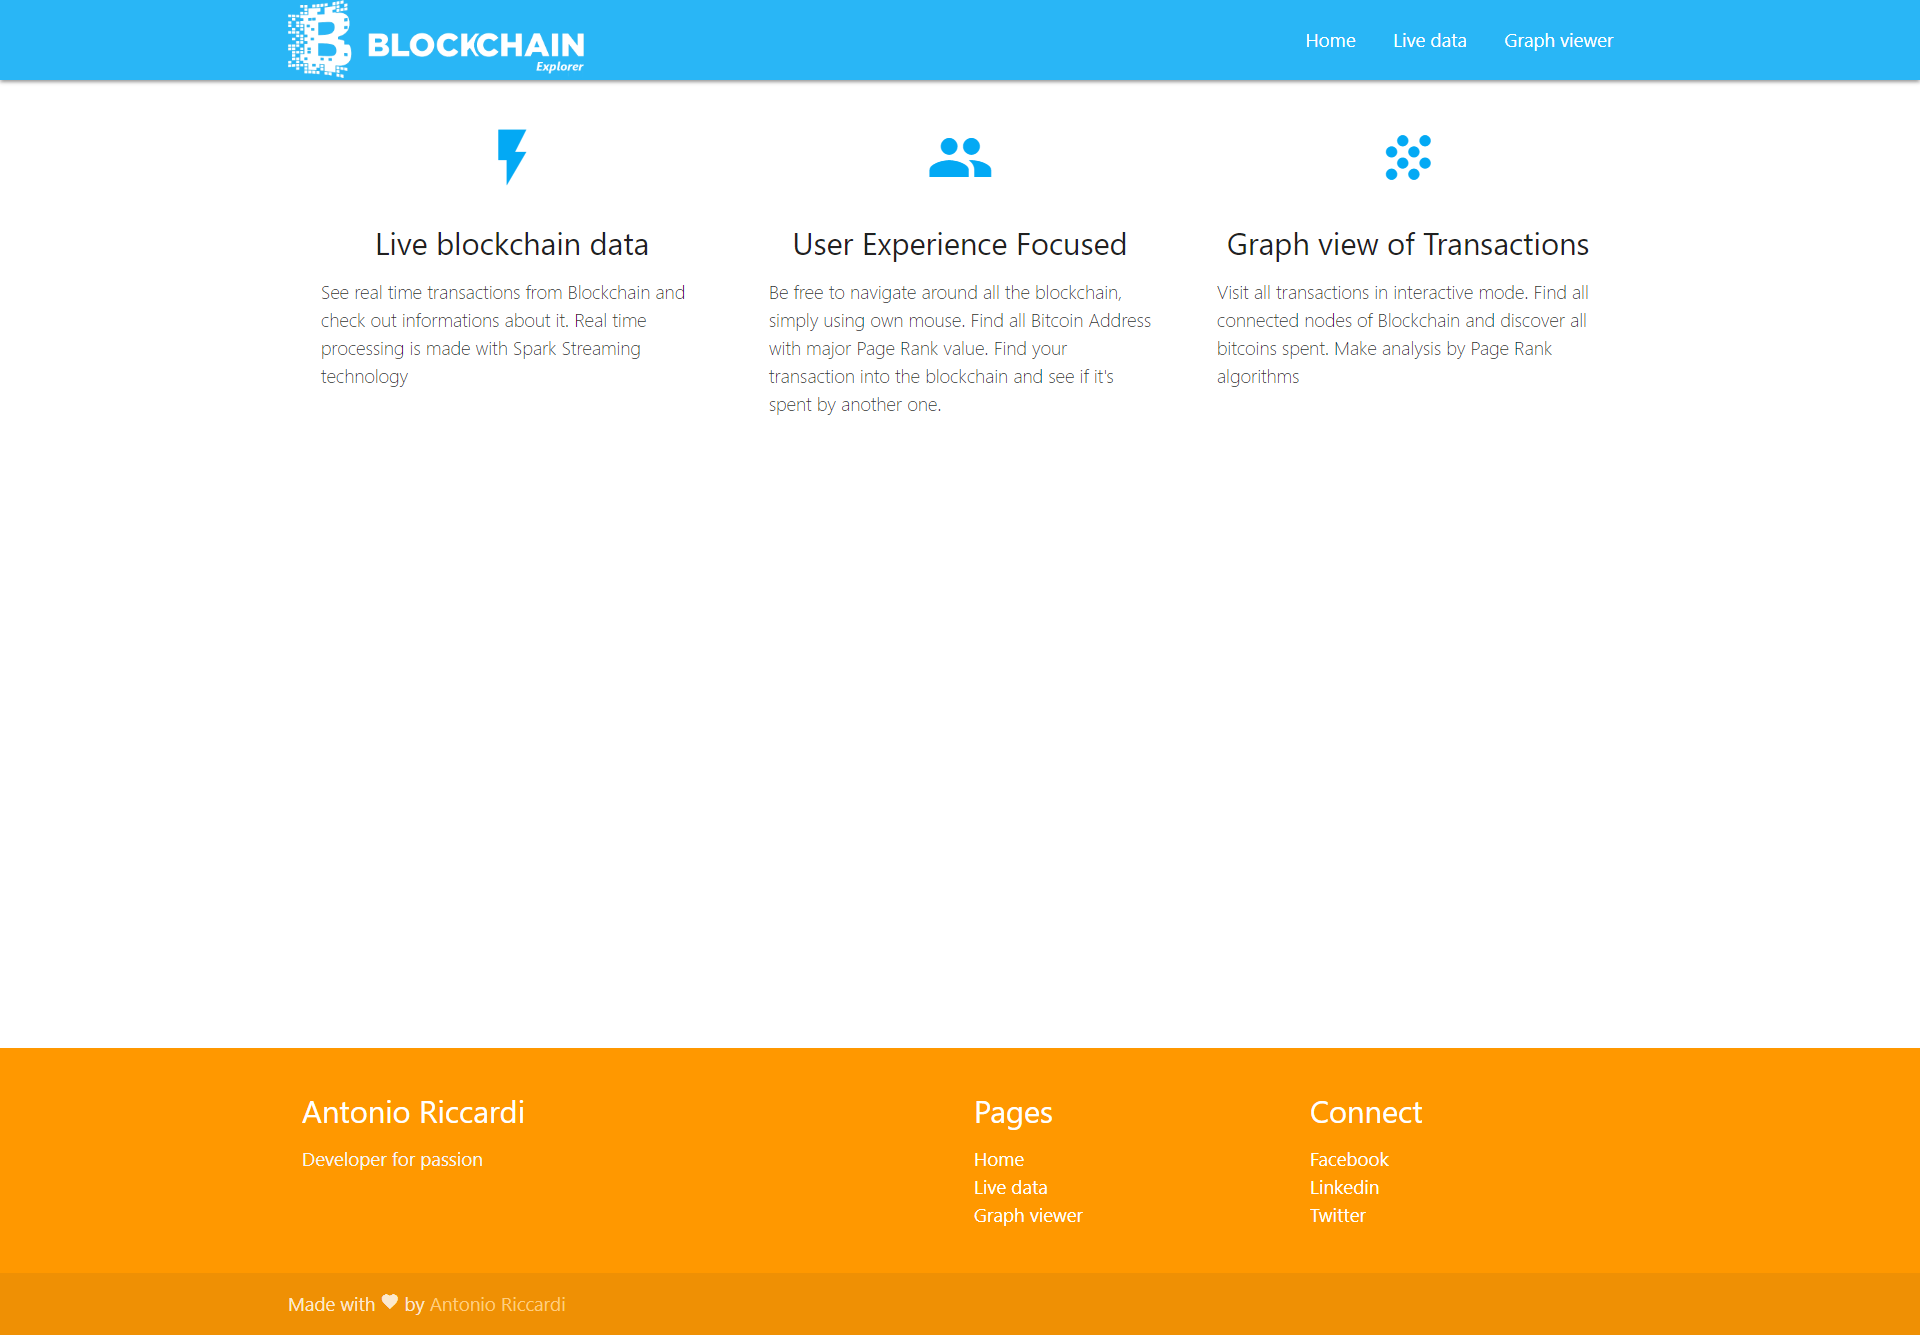
\includegraphics[width=\textwidth, height=0.60\textheight]{images/homePage.png}
	\caption{Home page Blockchain Explorer.}
	\label{fig:homePage}
\end{figure}
In questa prima pagina sono sintetizzate le principali funzionalità offerte dal sito,